% -*- coding: utf-8 -*-
\documentclass{article}
\usepackage{listings}
\usepackage{ctex}
\usepackage{graphicx}
\usepackage[a4paper, body={18cm,22cm}]{geometry}
\usepackage{amsmath,amssymb,amstext,wasysym,enumerate,graphicx}
\usepackage{float,abstract,booktabs,indentfirst,amsmath}
\usepackage{array}
\usepackage{booktabs} %调整表格线与上下内容的间隔
\usepackage{multirow}
\usepackage{diagbox}
\usepackage{hyperref}
\renewcommand\arraystretch{1.4}
\usepackage{indentfirst}
\setlength{\parindent}{2em}
\usepackage{graphbox}
\geometry{left=2.8cm,right=2.2cm,top=2.5cm,bottom=2.5cm}
%\geometry{left=3.18cm,right=3.18cm,top=2.54cm,bottom=2.54cm}

\graphicspath{{figures/}}

\title{\heiti 系统软件综合训练——银行家算法模拟系统之需求分析 }

\begin{document}
	
	\maketitle
	
	\vspace{5cm}
	
	\begin{table}[h]
		\centering
		\begin{Large}
			\begin{tabular}{p{3cm} p{7cm}<{\centering}}
				学 \qquad 校: &  安徽大学     \\ \cline{2-2}
				学 \qquad 院: & 计算机科学与技术学院   \\ \cline{2-2}
				学 \qquad 号: & X02014156   \\ \cline{2-2}
				姓 \qquad 名: & 凌兴 \\ \cline{2-2}
			\end{tabular}
		\end{Large}     
	\end{table}
	
	\newpage
	\renewcommand*\contentsname{\centering 目录 }
	\tableofcontents
	
	\newpage
	
	\section{需求分析}
		{\large
			需求分析部分主要确定系统需要具备的功能、逻辑模型和所含数据对象
		}
		\subsection{系统流程分析}
		{\normalsize
			在系统运行后等待用户输入客户数和资源数,接收到数据后随机生成银行所有资源的上限值、每个客户所需资源类数和个数、每类资源需要占用的时间、当前银行已分配给每个用户的资源,在此之后依照系统初始值生成尽可能多的安全序列,并按完成时间排序后显示到用户界面。
		}
		\subsection{系统功能分析与功能模块图}
			\subsubsection{系统初始化模块}
				{\small
					在接收到客户数和资源数后,以一定的约束随机生成银行所有资源的上限值、每个客户所需资源类数和个数、每类资源需要占用的时间、当前银行已分配给每个用户的资源。
				}
			\subsubsection{安全序列生成模块}
				{\small
					根据系统初始化模块产生的结果,为客户分配资源和回收资源,并以此产生一系列的安全序列。
				}
			\subsubsection{功能模块图}
				{\centering
					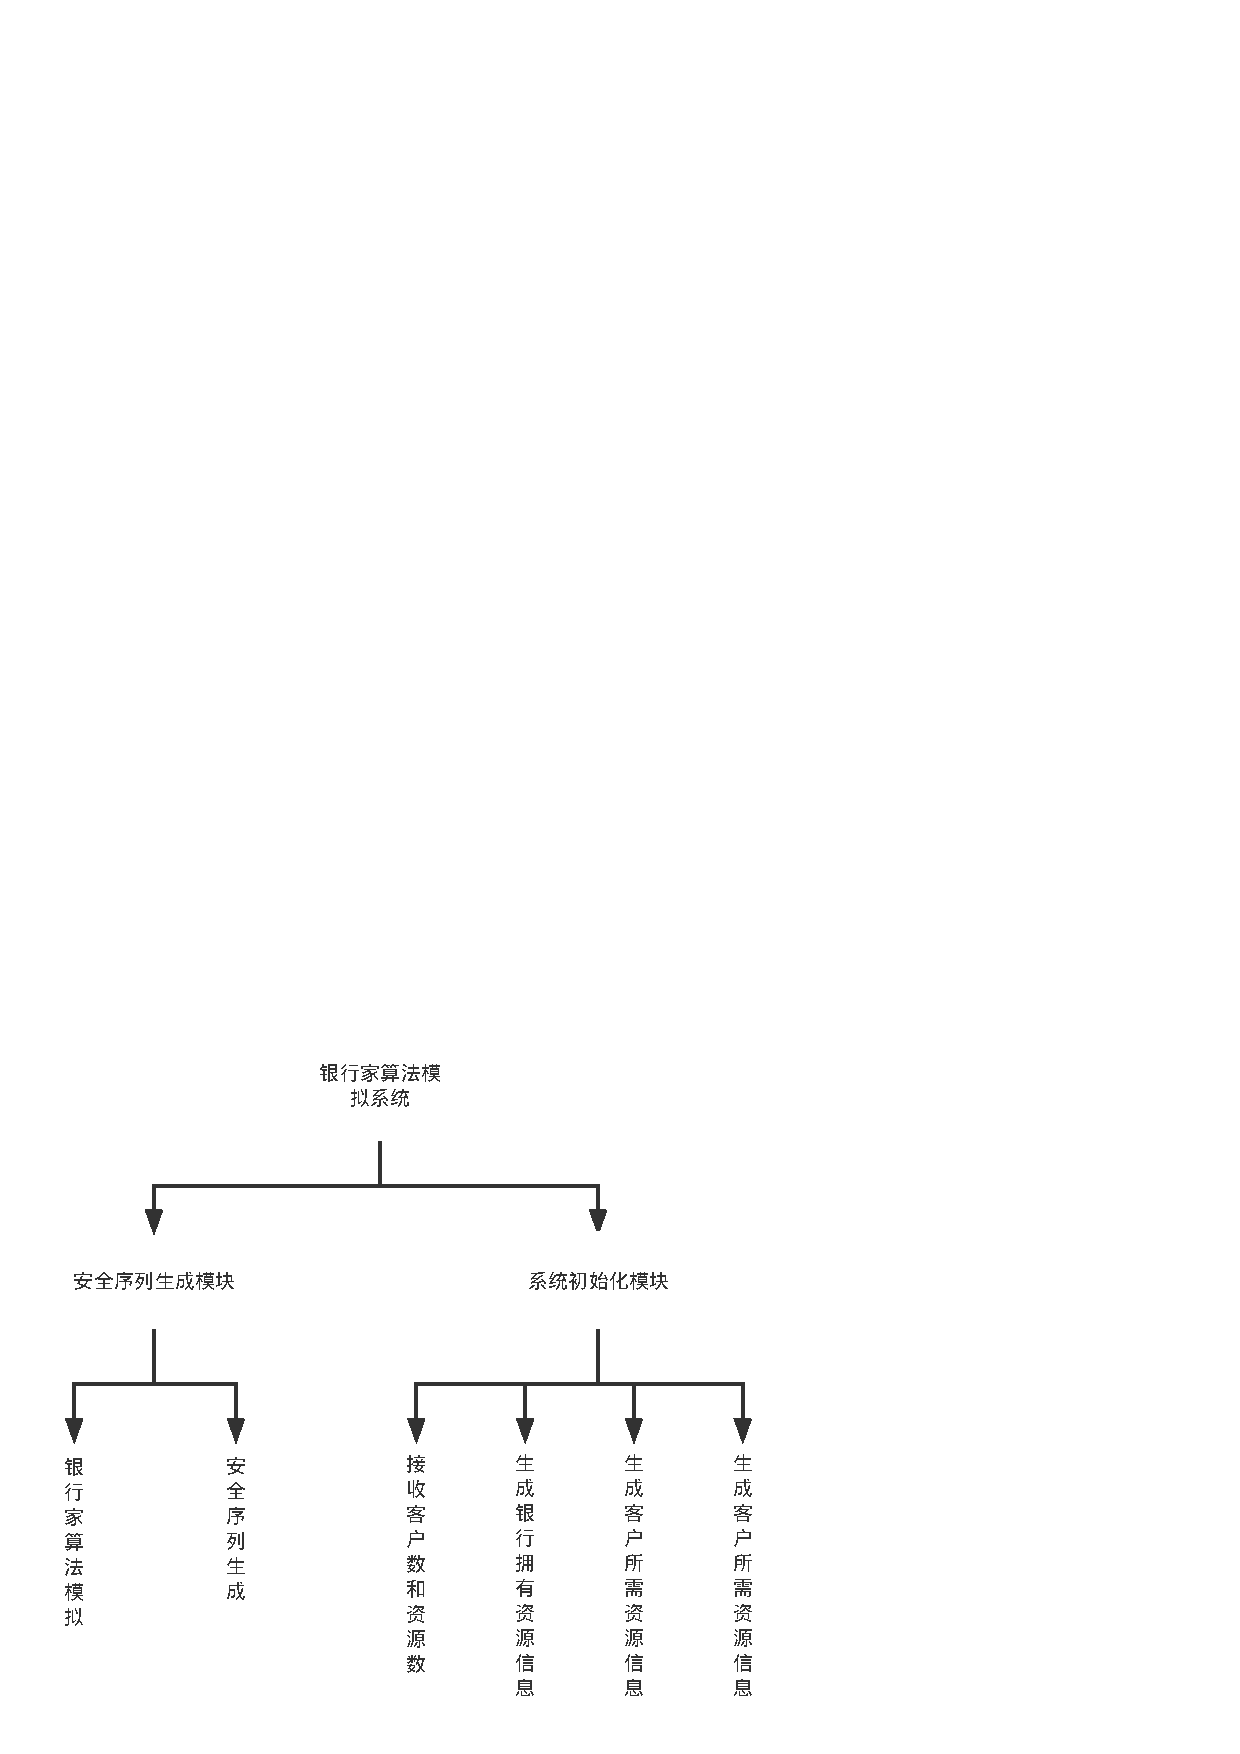
\includegraphics[align=c,width=\textwidth,height=\textheight/2]{模块功能图.pdf}
				}	
		\subsection{状态转换图}
			{\centering
				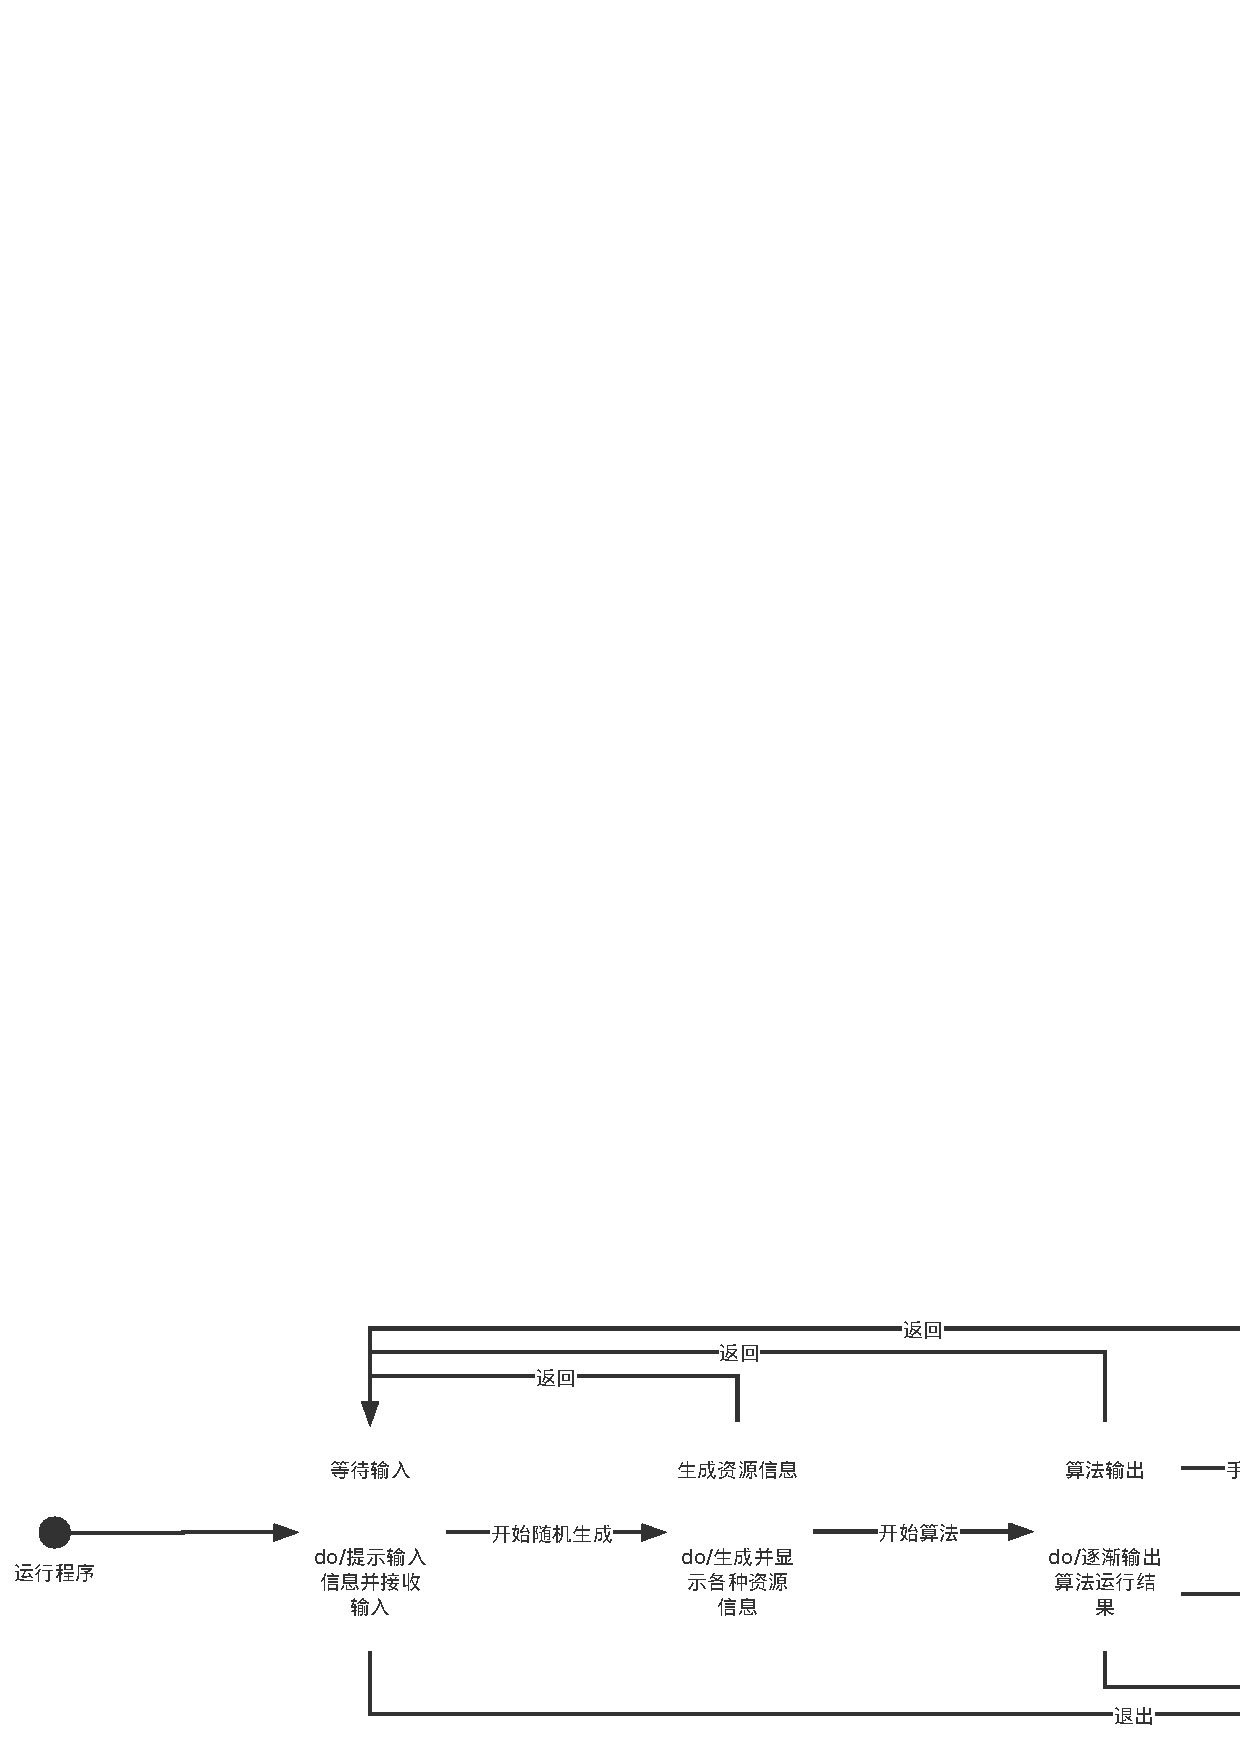
\includegraphics[align=c,width=\textwidth]{状态图.pdf}
			}\label{subsec:}

	\subsection{数据结构定义}
			采用面向对象的的思想,将系统中数据结构定义为如下几个类。
			\subsubsection{银行类}
			银行类包括资源表和客户表两个子成员变量,资源表存放银行剩余可用的资源,客户表存放需要提供资源的客户。
				~\\
				{\centering
					\includegraphics[align=c,width=\textwidth]{数据结构_银行类.pdf}
				}
			\subsubsection{客户类}
			客户类包括需求资源表、已有资源表和资源所需时间表,需求资源表存放总共需要的资源数,已有资源表存放当前拥有的资源数,资源所需时间表存放需要占用每类资源的时间。
				~\\
				~\\
				~\\
				{\centering
					\includegraphics[align=c,width=\textwidth]{数据结构_客户类.pdf}
				}
			\subsubsection{资源类}
			资源类包括资源类型名,资源类型名存放当前资源的类型。
				~\\
				~\\
				~\\
				{\centering
					\includegraphics[width=\columnwidth,align=c]{数据结构_资源类.pdf}
				}
\end{document}

%%%%%%%%%%%%%%%%%%%%%%%%%%%%Library%%%%%%%%%%%%%%%%%%%%%%%%%%%%%%%%%%%%%%%

% 1. 脚注用法
LaTeX\footnote{Latex is Latex} is a good software

%2. 强调
\emph{center of percussion} %[Brody 1986], %\lipsum[5]

%3. 随便生成一段话
\lipsum[4]

%4. 列条目
\begin{itemize}
	\item the angular velocity of the bat,
	\item the velocity of the ball, and
	\item the position of impact along the bat.
\end{itemize}

%5. 表格用法
\begin{table}[h]
	\centering  
	\begin{tabular}{c|cc}
		\hline
		年份 & \multicolumn{2}{c}{指标}\\
		\hline
		2017 & 0.9997 & 0.0555 \\
		2018 & 0.9994 & 0      \\
		2019 & 0.9993 & 0      \\
		\hline
	\end{tabular}
	\caption{NAME}\label{SIGN}
\end{table}

\begin{center}
	\begin{tabular}{c|cclcrcc}
		\hline
		Year & theta & $S_1^-$ & $S_2^-$ & $S_3^-$ & $S_4^+$ & $S_5^+$ & $S_6^+$ \\%表格标题
		\hline
		2016 & 1      & 0      & 0 & 0.0001 & 0      & 0      & 0 \\
		2017 & 0.9997 & 0.0555 & 0 & 0.2889 & 0.1844 & 0.463  & 0 \\
		2018 & 0.9994 & 0      & 0 & 0.0012 & 0.3269 & 0.7154 & 0 \\
		2019 & 0.9993 & 0      & 0 & 0      & 0.4325 & 1.0473 & 0 \\
		2020 & 0.9991 & 0      & 0 & 0      & 0.5046 & 1.2022 & 0 \\
		2021 & 0.999  & 0      & 0 & 0      & 0.5466 & 1.2827 & 0 \\
		2022 & 0.9989 & 0.0017 & 0 & 0.3159 & 0.562  & 1.2995 & 0 \\
		2023 & 0.9989 & 0      & 0 & 0.0109 & 0.5533 & 1.2616 & 0 \\
		2024 & 0.9989 & 0      & 0 & 0      & 0.5232 & 1.1769 & 0 \\
		2025 & 0.9989 & 0      & 0 & 0.1009 & 0.4738 & 1.0521 & 0 \\
		2026 & 0.9991 & 0      & 0 & 0      & 0.4071 & 0.8929 & 0 \\
		2027 & 0.9992 & 0.0004 & 0 & 0.1195 & 0.3248 & 0.7042 & 0 \\
		2028 & 0.9994 & 0.0164 & 0 & 0.046  & 0.2287 & 0.4902 & 0 \\
		2029 & 0.9997 & 0      & 0 & 0.0609 & 0.12   & 0.2545 & 0 \\
		2030 & 1      & 0      & 0 & 0      & 0      & 0      & 0 \\
		\hline
	\end{tabular}
\end{center}

%6. 数学公式
\begin{equation}
	a^2 = a * a\label{aa}
\end{equation}

\[
\begin{pmatrix}{*{20}c}
	{a_{11} } & {a_{12} } & {a_{13} }  \\
	{a_{21} } & {a_{22} } & {a_{23} }  \\
	{a_{31} } & {a_{32} } & {a_{33} }  \\
\end{pmatrix}
= \frac{{Opposite}}{{Hypotenuse}}\cos ^{ - 1} \theta \arcsin \theta
\]

\[
p_{j}=\begin{cases} 0,&\text{if $j$ is odd}\\
	r!\,(-1)^{j/2},&\text{if $j$ is even}
\end{cases}
\]


\[
\arcsin \theta  =
\mathop{{\int\!\!\!\!\!\int\!\!\!\!\!\int}\mkern-31.2mu
	\bigodot}\limits_\varphi
{\mathop {\lim }\limits_{x \to \infty } \frac{{n!}}{{r!\left( {n - r}
			\right)!}}} \eqno (1)
\]

%7. 双图并行
\begin{figure}[h]
	% 一个2*2图片的排列
	\begin{minipage}[h]{0.5\linewidth}
		\centering
		\includegraphics[width=0.8\textwidth]{./figures/0.jpg}
		\caption{Figure example 2}
	\end{minipage}
	\begin{minipage}[h]{0.5\linewidth}
		\centering
		\includegraphics[width=0.8\textwidth]{./figures/0.jpg}
		\caption{Figure example 3}
	\end{minipage}
\end{figure}

%8. 单张图片部分
\begin{figure}[h]
	%\small
	\centering
	\includegraphics[width=12cm]{./figures/mcmthesis-aaa.eps}
	\caption{Figure example 1} \label{fig:aa}
\end{figure}

%%%%%%%%%%%%%%%%%%%%%%%%%%%%%%%%%%%%%%%%%%%%%%%%%%%%%%%%%%%%%%%%%%%%%%%%%%%%%
\begin{minipage}{0.5\linewidth}
	\begin{tabular}{|c|c|c|}
		\hline
		\multicolumn{2}{|c|}{\multirow{2}{*}{合并}}&测试\\
		\cline{3-3}
		\multicolumn{2}{|c|}{}& 0.9997  \\
		\hline
		2019 & 0.9993 & 0 \\
		\hline
	\end{tabular}
\end{minipage}

\begin{minipage}{0.5\linewidth}
	\begin{tabular}{c|ccc}
		\hline
		年份 & \multicolumn{3}{c}{指标}\\
		\hline
		\multirow{3}{*}{合并}&2017 & 0.9997 & 0.0555 \\
		&2018 & 0.9994 & 0      \\
		&2019 & 0.9993 & 0      \\
		\hline
	\end{tabular}
\end{minipage}



\begin{table}[h]
	\centering  
	\begin{Large}
		\begin{tabular}{p{4cm} p{8cm} < {\centering}}
			\hline
			院\qquad 系: & 信息工程学院 \\
			\hline
			团队名称: & PlantBook Team \\
			\hline
			分\qquad 组: & 第0组1号 \\
			\hline
			日\qquad 期: & 2017年10月28日 \\
			\hline
			指导教师: & 吱吱吱\\
			\hline
		\end{tabular}
	\end{Large}
\end{table}


\ctexset{
	section={
		format+=\heiti \raggedright,
		name={,、},
		number=\chinese{section},
		beforeskip=1.0ex plus 0.2ex minus .2ex,
		afterskip=1.0ex plus 0.2ex minus .2ex,
		aftername=\hspace{0pt}
	},
}

\begin{table}[h]
	\centering
	\begin{Large}
		\begin{tabular}{p{3cm} p{7cm}<{\centering}}
			院  \qquad  系: & 信息工程学院           \\ \cline{2-2}
		\end{tabular}
	\end{Large}     
\end{table}
\thispagestyle{empty}
\newpage
\thispagestyle{empty}
\tableofcontents
\thispagestyle{empty}
\newpage
\setcounter{page}{1}

% 9. 代码

\usepackage{listings}
\usepackage{xcolor}
\lstset{
	numbers=left, 
	numberstyle= \tiny, 
	keywordstyle= \color{ blue!70},
	commentstyle= \color{red!50!green!50!blue!50}, 
	frame=shadowbox, % 阴影效果
	rulesepcolor= \color{ red!20!green!20!blue!20} ,
	escapeinside=``, % 英文分号中可写入中文
	xleftmargin=2em,xrightmargin=2em, aboveskip=1em,
	basicstyle=\footnotesize,
	framexleftmargin=2em
}